\begin{figure*}[t]
\centering
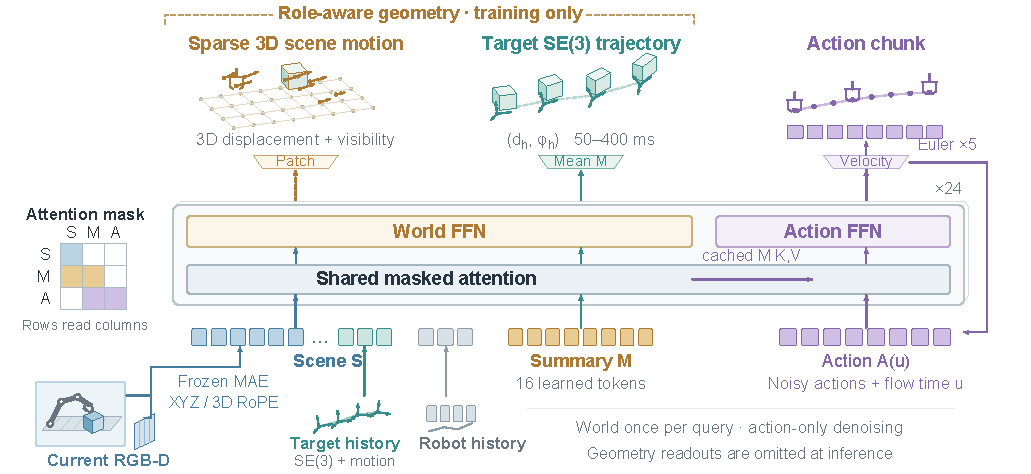
\includegraphics[width=\textwidth]{figures/Fig2/fig2_se3wam.pdf}
\caption{\textbf{\ours architecture.}
(a) Read bottom to top. Current RGB-D and target/robot histories form scene tokens $S$;
16 learned summaries $M$ complete the world stream.
The 12-layer backbone shares attention projections and uses separate world/action FFNs.
Training-only readouts (dashed) predict sparse scene displacement and visibility from patch states,
and target SE(3) trajectories from the mean summary; auxiliary targets are listed below the geometric panels.
The geometric examples are recorded labels at 3 of 8 horizons spanning 50--400\,ms:
gray glyphs mark current poses and orange glyphs future poses (glyph size illustrative);
displacement arrows on the current point cloud are magnified $3\times$.
Action icons are schematic.
(b) Mask rows are queries and columns are keys: $S$ reads $S$, $M$ reads $S,M$,
and $A$ reads $S,M,A$. Actions read world hidden states.
(c) Inference skips forecast readouts and caches world keys and values once per query
for \cfgEuler{} Euler action steps.}
\label{fig:architecture}
\end{figure*}
